% Paquets généraux
\documentclass[a4paper,12pt,titlepage,twoside]{article}
\usepackage[T1]{fontenc}
\usepackage[utf8]{inputenc}
\usepackage[french]{babel}
\usepackage[gen]{eurosym}
%\usepackage[dvips]{graphicx}
\usepackage{fancyhdr}
\usepackage{pdfpages} 
\usepackage{multido}
\usepackage{enumitem}
\usepackage{hyperref}
%\usepackage{textcomp}
%\usepackage{aeguill}
\usepackage{schemabloc}
\usepackage[bitstream-charter]{mathdesign}

\newcommand{\id}{30}
\newcommand{\nom}{Calculs d'hyperstatisme}
\newcommand{\sequence}{04}
\newcommand{\nomsequence}{Liaisons entre les solides}
\newcommand{\num}{03}
\newcommand{\type}{TD}
\newcommand{\descrip}{En appliquant les règles de la théorie des mécanisme, déterminer le degré d'hyperstatisme de plusieurs systèmes et proposer des solutions afin de diminuer ce degré}
\newcommand{\competences}{B2-12: Proposer une modélisation des liaisons avec leurs caractéristiques géométriques. \\ &  B2-13: Proposer un modèle cinématique paramétré à partir d'un système réel, d'une maquette numérique ou d'u \\ &  B2-17: Simplifier un modèle de mécanisme. \\ &  B2-18: Modifier un modèle pour le rendre isostatique.}
\newcommand{\nbcomp}{4}
\newcommand{\systemes}{E.P.A.S, Machine d'essai de traction}
\newcommand{\systemesnum}{14, 13}
\newcommand{\systemessansaccent}{E.P.A.S, Machine d'essai de traction}
\newcommand{\ilot}{3}
\newcommand{\ilotstr}{03}
\newcommand{\dossierilot}{\detokenize{Ilot_03 E.P.A.S, Machine d'essai de traction}}
\newcommand{\imageun}{EPAS}
\newcommand{\imagedeux}{Machine_dessai_de_traction}


\newcommand{\institute}{Lycée Dorian}


\usepackage{color}
\usepackage{xcolor}
\usepackage{colortbl}
\usepackage{helvet}
\renewcommand{\familydefault}{\sfdefault}
\usepackage[frenchmath]{newtxsf} % for sans serif symbols
%\usepackage{amsfonts}
%\usepackage{amsmath}
%\usepackage{xspace}
\usepackage{varioref}
\usepackage{tabularx}
%\usepackage{floatflt}
\usepackage{graphics}
\usepackage{wrapfig}
\usepackage{textcomp}
\usepackage{tikz}
\usepackage{wrapfig}
\usepackage{gensymb}
\usepackage[european]{circuitikz}
\usetikzlibrary{babel}
\usepackage{ifthen}
\usepackage{cancel}
\usepackage{etoolbox}
\usepackage{multirow}
%\usepackage{boxedminipage}
\definecolor{gris25}{gray}{0.75}
\definecolor{bleu}{RGB}{18,33,98}
\definecolor{bleuf}{RGB}{42,94,171}
\definecolor{bleuc}{RGB}{231,239,247}
\definecolor{rougef}{RGB}{185,18,27}
\definecolor{rougec}{RGB}{255,188,204}%255,230,231
\definecolor{vertf}{RGB}{103,126,82}
\definecolor{vertc}{RGB}{220,255,191}
\definecolor{forestgreen}{rgb}{0.13,0.54,0.13}
\definecolor{blcr}{rgb}{0.59,0.69,0.84}
\definecolor{blfr}{rgb}{0.32,0.51,0.75}
\definecolor{orfr}{rgb}{0.90,0.42,0.15}
\definecolor{orcr}{rgb}{0.90,0.65,0.50}
\definecolor{orangef}{rgb}{0.659,0.269,0.072}
\definecolor{orange}{rgb}{0.58,0.35,0.063}
\definecolor{orangec}{rgb}{0.43,0.32,0.25}
\definecolor{rcorrect}{rgb}{0.6,0,0}
\definecolor{sequence}{rgb}{0.75,0.75,0.75}
\definecolor{competences}{rgb}{0.61,0.73,0.35}
\definecolor{grisf}{HTML}{222222}
\definecolor{grisc}{HTML}{636363}
\definecolor{normal}{HTML}{4087c4}
\definecolor{info}{HTML}{5bc0de}
\definecolor{success}{RGB}{92,184,92}
\definecolor{warning}{RGB}{240,173,78}
\definecolor{danger}{RGB}{217,83,79}
\hypersetup{                    % parametrage des hyperliens
    colorlinks=true,                % colorise les liens
    breaklinks=true,                % permet les retours à la ligne pour les liens trop longs
    urlcolor= blfr,                 % couleur des hyperliens
    linkcolor= orange,                % couleur des liens internes aux documents (index, figures, tableaux, equations,...)
    citecolor= forestgreen                % couleur des liens vers les references bibliographiques
    }

% Mise en page
\pagestyle{fancy}

\setlength{\hoffset}{-18pt}

\setlength{\oddsidemargin}{0pt} 	% Marge gauche sur pages impaire2s
\setlength{\evensidemargin}{0pt} 	% Marge gauche sur pages paires
\setlength{\marginparwidth}{00pt} 	% Largeur de note dans la marge
\setlength{\headwidth}{481pt} 	 	% Largeur de la zone de tête (17cm)
\setlength{\textwidth}{481pt} 	 	% Largeu\textbf{r de la zone de texte (17cm)
\setlength{\voffset}{-18pt} 		% Bon pour DOS
\setlength{\marginparsep}{7pt}	 	% Séparation de la marge
\setlength{\topmargin}{-30pt} 		% Pas de marge en haut
\setlength{\headheight}{35pt} 		% Haut de page
\setlength{\headsep}{20pt} 		% Entre le haut de page et le texte
\setlength{\footskip}{30pt} 		% Bas de\textbf{ page + séparation
\setlength{\textheight}{700pt} 		% Hauteur de l'icone zone de texte (25cm)
\setlength\fboxrule{1 pt}
\renewcommand{\baselinestretch}{1}
\setcounter{tocdepth}{1}
\newcommand{\cadre}[2]
{\fbox{
  \begin{minipage}{#1\linewidth}
   \begin{center}
    #2\\
   \end{center}
  \end{minipage}
 }
}

\newcounter{num_quest} \setcounter{num_quest}{0}
\newcounter{num_rep} \setcounter{num_rep}{0}
\newcounter{num_cor} \setcounter{num_cor}{0}

\newcommand{\question}[1]{\refstepcounter{num_quest}\par
~\ \\ \textbf{Question \arabic{num_quest} : }#1\label{q\the\value{num_quest}}\par
}


\newcommand{\feuilleDR}[1]{
	\begin{tikzpicture}
		\draw[gray!30](0,0)grid[step=0.5cm](\linewidth,#1);
	\end{tikzpicture}
}


\newcommand{\reponse}[4][1]
{\noindent
\parbox{\textwidth}{
\rule{\linewidth}{.5pt}\\
\textbf{Question\ifthenelse{#1>1}{s}{} \multido{}{#1}{%
\refstepcounter{num_rep}\ref{q\the\value{num_rep}} }:} ~\ \\
\ifdef{\public}{#3 \ifthenelse{#2>0}{~\ \\ 	\feuilleDR{#2}}}{#4}
}}

\newcommand{\cor}
{\refstepcounter{num_cor}
\noindent
\rule{\linewidth}{.5pt}
\textbf{Question \arabic{num_cor}:} \\
}

\newcommand{\titre}[1]
{\begin{center}
\cadre{0.8}{\huge #1} 
\end{center}
}

\newcommand{\finsujet}
{
    \begin{center}
    \Large{FIN}
    \end{center}

    \cleardoublepage

	\def\public

    \ifdef{\public}{\pagestyle{docreponse}}{\pagestyle{correction}}

    \ifdef{\public}{
        \begin{tikzpicture} 
            \draw (0,0) rectangle (2,2);
            \draw (0,0) -- (2,2);
            \draw (1.5,0.5) node {\large 20};
            \draw (2.5,0) rectangle (16,2);
            \draw (4.5,1.7) node {\large Commentaires:};
        \end{tikzpicture}
        \ifdefined\competences
	      ~\ \\ ~\ \\
	      \centering
		  \foreach \competence in \competences
		  {
			\fbox{\begin{tikzpicture} 
			\draw (0,0) circle[radius=0.5];
		    \node at (0.5,0) [anchor=west] {\competence};
   	     \end{tikzpicture}
   	    	}
   	    }
	   	\fi
	   	 ~\ \\
	}

    ~\ \\
}

% En tête et pied de page
\fancypagestyle{normal}{%
\fancyhf{}
\lhead{\sujet}
\rhead{\includegraphics[width=2cm]{../../../img/logo}\hspace{2pt}}
\ifdef{\auteurdeux}{\lfoot{\auteurun,\ \auteurdeux}}{\lfoot{\auteurun}}
\rfoot{\nom}
}

\fancypagestyle{docreponse}{%
\fancyhf{}
\fancyhead[LO]{NOM Prénom: .............................}
\rhead{\includegraphics[width=2cm]{../../../img/logo}\hspace{2pt}}
\ifdef{\auteurdeux}{\lfoot{\auteurun,\ \auteurdeux}}{\lfoot{\auteurun}}
\rfoot{\nom}
}

\fancypagestyle{correction}{%
  \fancyhf{}
  \lhead{\colorbox{danger}{\begin{minipage}{0.65\paperwidth} \textcolor{white}{\textbf{Correction}} \end{minipage}} }
  \rhead{\includegraphics[width=2cm]{../../../img/logo}}
  \ifdef{\auteurdeux}{\lfoot{\auteurun,\auteurdeux}}{\lfoot{\auteurun}}
  \rfoot{\colorbox{danger}{\begin{minipage}{0.5\paperwidth} \begin{flushright}\textcolor{white}{\textbf{Correction}}\end{flushright} \end{minipage}} }}

\renewcommand{\footrulewidth}{0.4pt}

\usepackage{eso-pic}
\newcommand{\BackgroundPic}{%
\put(0,0){%
\parbox[b][\paperheight]{\paperwidth}{%
\vfill
\begin{center}
\hspace{0.5cm}\vspace{0.5cm}
\includegraphics[width=\paperwidth,height=\paperheight,%
keepaspectratio]{../../../img/fond3}%
\end{center}
\vfill
}}}

\newcommand{\BackgroundPicdeux}{%
\put(25,-30){%
\parbox[b][\paperheight]{\paperwidth}{%
\vfill
\begin{center}
\includegraphics[width=\paperwidth,height=\paperheight,%
keepaspectratio]{../../../img/fond4}%
\end{center}
\vfill
}}}

\begin{document}

\AddToShipoutPicture{\BackgroundPicdeux}

\pagestyle{normal}


\section{Lève vitre électrique}

\subsection{Présentation du système}

\begin{minipage}{0.48\linewidth}
 \centering\includegraphics[width=0.5\linewidth]{img/leve_vitre_auto}
\end{minipage}
\hfill
\begin{minipage}{0.48\linewidth}
Les vitres électriques sont mises en mouvement grâce à un moteur électrique en rotation. C'est le système que nous étudions ici qui permet de transformer ce mouvement de rotation en translation de la vitre.
\end{minipage}

\section{Etude de la vitesse du déplacement de la vitre}


\begin{minipage}{0.38\linewidth}
Le mouvement d'entrée est la rotation de $1$ par rapport à $0$, la vitesse est donc $\omega_{1/0}$ indiquée sur la figure ci-contre.

Données géométriques:
\begin{itemize}
 \item $\overrightarrow{AE}=L.\overrightarrow{x_1}$,
 \item $\overrightarrow{AB}=L.cos(\theta_1).\overrightarrow{x_0}$,
 \item $\overrightarrow{AD}=L.sin(\theta_1).\overrightarrow{y_0}$,
 \item $\overrightarrow{AC}=\dfrac{L}{2}.\overrightarrow{x_1}$,
 \item $\overrightarrow{DG}=\dfrac{L}{2}.cos(\theta_1).\overrightarrow{x_0}+e.\overrightarrow{y_0}$,
\end{itemize}
\end{minipage}
\hfill
\begin{minipage}{0.58\linewidth}
 \centering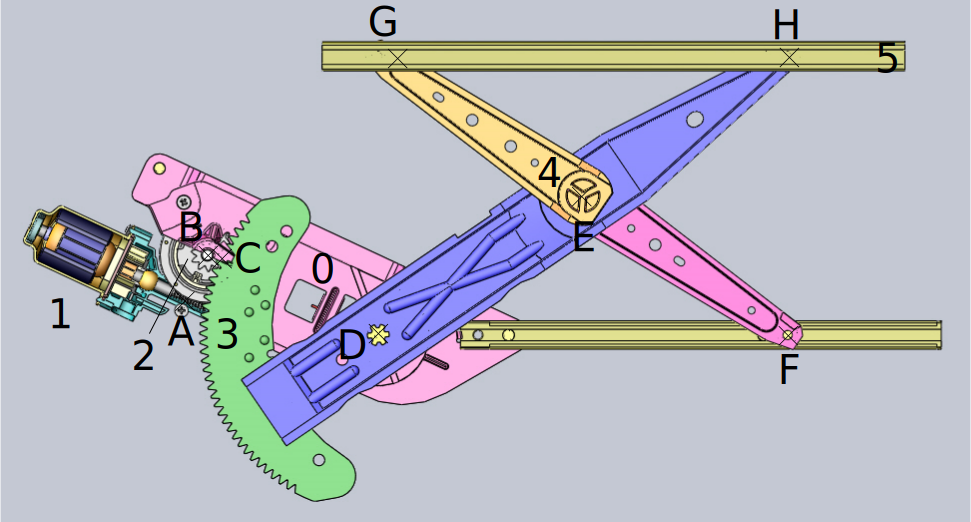
\includegraphics[width=0.9\linewidth]{img/leve_vitre}
\end{minipage}

~\

Les liaisons aux points A, C et D sont des liaisons pivots et celles en B et E sont des liaisons ponctuelles.

\question{Dessiner le graphe de liaison de ce système.}

\question{Donner les torseurs cinématiques suivants:
\begin{itemize}
 \item $\left\{V_{1/0}\right\}$ de la liaison entre la pièce $1$ et le bâti $0$ en $A$,
 \item $\left\{V_{2/1}\right\}$ de la liaison entre la pièce $2$ et le bâti $1$ en $C$,
 \item $\left\{V_{2/0}\right\}$ de la liaison entre la pièce $2$ et le bâti $0$ en $B$,
 \item $\left\{V_{3/2}\right\}$ de la liaison entre la pièce $3$ et le bâti $2$ en $D$,
 \item $\left\{V_{3/1}\right\}$ de la liaison entre la pièce $3$ et le bâti $1$ en $E$.
\end{itemize} 
}

\question{Déplacer le torseur cinématique $\left\{V_{2/1}\right\}$ de la liaison entre la pièce $2$ et le bâti $1$ du point $C$ au point $A$.}

\question{Déplacer le torseur cinématique $\left\{V_{2/0}\right\}$ de la liaison entre la pièce $2$ et le bâti $0$ du point $B$ au point $A$.}

\section{Questions bonus à faire à la maison}

\question{Déplacer le torseur cinématique $\left\{V_{3/2}\right\}$ de la liaison entre la pièce $3$ et le bâti $2$ du point $D$ au point $A$.}

\question{Déplacer le torseur cinématique $\left\{V_{3/1}\right\}$ de la liaison entre la pièce $3$ et le bâti $1$ du point $E$ au point $A$.}

Une des deux relations torsorielles nécessaires afin de résoudre le comportement de ce système est $\left\{V_{3/1}\right\}_{A,R_0}+\left\{V_{1/0}\right\}_{A,R_0}=\left\{V_{3/2}\right\}_{A,R_0}+\left\{V_{2/0}\right\}_{A,R_0}$.

\question{Déterminer une autre relation torsorielle complémentaire.}

\question{Écrire le système d'équations qui lie les composantes des torseurs cinématiques issu des ces deux relations torsorielles.}

\question{En déduire la vitesse $\overrightarrow{V_{E\in 3/1}}$ en fonction de $\omega_{1/0}$, $\theta_1$ et $L$.}

Rappels:

On notera le torseur cinématique du solide i par rapport au solide j exprimé au point M par :

\begin{center}
\begin{math}
\left\{V_{i/j}\right\}=\left\{
\begin{array}{cc}
\omega_{x,ij} & V_{x,M,ij} \\
\omega_{y,ij} & V_{y,M,ij} \\
\omega_{z,ij} & V_{z,M,ij}
\end{array}
\right\}_{X,R_P}
\end{math}, avec $R_P=(\overrightarrow{X_P},\overrightarrow{Y_P},\overrightarrow{Z_P})$
\end{center}

\finsujet

\reponse{6}{}{
\begin{center}
\def\svgwidth{.6\linewidth}
\input{img/graphe_liaison.pdf_tex}
\end{center}
}

\reponse{6}{}{
$\left\{V_{1/0}\right\}=\left\{
\begin{array}{cc}
0 & 0 \\
0 & 0 \\
\omega_{10} & 0
\end{array}
\right\}_{A}$
$\left\{V_{2/1}\right\}=\left\{
\begin{array}{cc}
0 & 0 \\
0 & 0 \\
\omega_{21} & 0
\end{array}
\right\}_{C}$
$\left\{V_{2/0}\right\}=\left\{
\begin{array}{cc}
\omega_{x,20} & V_{x,20} \\
\omega_{y,20} & 0 \\
\omega_{z,20} & V_{z,20}
\end{array}
\right\}_{B}$
$\left\{V_{3/2}\right\}=\left\{
\begin{array}{cc}
0 & 0 \\
0 & 0 \\
\omega_{32} & 0
\end{array}
\right\}_{D}$
$\left\{V_{3/1}\right\}=\left\{
\begin{array}{cc}
\omega_{x,31} & V_{x,31} \\
\omega_{y,31} & 0 \\
\omega_{z,31} & V_{z,31}
\end{array}
\right\}_{E}$
}

\reponse{6}{}{
\begin{math}
\left\{V_{2/1}\right\}=\left\{
\begin{array}{cc}
0 & 0 \\
0 & 0 \\
\omega_{21} & 0
\end{array}
\right\}_{C}=\left\{
\begin{array}{cc}
0 & \dfrac{L}{2}.\omega_{21}.sin(\theta_1) \\
0 & -\dfrac{L}{2}.\omega_{21}.cos(\theta_1) \\
\omega_{21} & 0
\end{array}
\right\}_{A}
\end{math}
}

\reponse{6}{}{
\begin{math}
\left\{V_{2/0}\right\}=\left\{
\begin{array}{cc}
\omega_{x,20} & V_{x,20} \\
\omega_{y,20} & 0 \\
\omega_{z,20} & V_{z,20}
\end{array}
\right\}_{B}=\left\{
\begin{array}{cc}
\omega_{x,20} & V_{x,20} \\
\omega_{y,20} & -L.\omega_{z,20}.cos(\theta_1) \\
\omega_{z,20} & V_{z,20}+L.\omega_{y,20}.cos(\theta_1)
\end{array}
\right\}_{A}
\end{math}
}

\newpage

\reponse{6}{}{
\begin{math}
\left\{V_{3/2}\right\}=\left\{
\begin{array}{cc}
0 & 0 \\
0 & 0 \\
\omega_{32} & 0
\end{array}
\right\}_{D}=\left\{
\begin{array}{cc}
0 & L.\omega_{32}.sin(\theta_1) \\
0 & 0 \\
\omega_{32} & 0
\end{array}
\right\}_{A}
\end{math}
}

\reponse{6}{}{
\begin{math}
\left\{V_{3/1}\right\}=\left\{
\begin{array}{cc}
\omega_{x,31} & V_{x,31} \\
\omega_{y,31} & 0 \\
\omega_{z,31} & V_{z,31}
\end{array}
\right\}_{E}=\left\{
\begin{array}{cc}
\omega_{x,31} & V_{x,31}+L.\omega_{z,31}.sin(\theta_1) \\
\omega_{y,31} & -L.\omega_{z,31}.cos(\theta_1) \\
\omega_{z,31} & V_{z,31}+L.\omega_{y,31}.cos(\theta_1)-L.\omega_{x,31}.sin(\theta_1)
\end{array}
\right\}_{A}
\end{math}
}

\reponse{6}{}{
\begin{math} 
\left\{V_{2/0}\right\}=\left\{V_{2/1}\right\}+\left\{V_{1/0}\right\} ou 
\left\{V_{3/1}\right\}=\left\{V_{3/2}\right\}+\left\{V_{2/1}\right\}
\end{math}
}

\reponse{6}{}{
$\left\{V_{3/1}\right\}_{A,R_0}+\left\{V_{1/0}\right\}_{A,R_0}=\left\{V_{3/2}\right\}_{A,R_0}+\left\{V_{2/0}\right\}_{A,R_0}$

\begin{math}
\left\{
\begin{array}{l}
\omega_{x,31}=\omega_{x,20} \\
\omega_{y,31}=\omega_{y,20} \\
\omega_{z,31}+\omega_{10}=\omega_{32}+\omega_{z,20} \\
V_{x,31}+L.\omega_{z,31}.sin(\theta_1)=L.\omega_{32}.sin(\theta_1)+V_{x,20} \\
-L.\omega_{z,31}.cos(\theta_1)=-L.\omega_{z,20}.cos(\theta_1) \\
V_{z,31}+L.\omega_{y,31}.cos(\theta_1)-L.\omega_{x,31}.sin(\theta_1)=V_{z,20}+L.\omega_{y,20}.cos(\theta_1)
\end{array}\right.
\end{math}

\begin{math}
\left\{
\begin{array}{l}
\omega_{x,20}=0 \\
\omega_{y,20}=0 \\
\omega_{z,20}=\omega_{21}+\omega_{10} \\
V_{x,20}=\dfrac{L}{2}.\omega_{21}.sin(\theta1) \\
-L.\omega_{z,20}.cos(\theta1)=-\dfrac{L}{2}.\omega_{21}.cos(\theta1) \\
V_{z,20}+L.\omega_{y,20}.cos(\theta1)=0
\end{array}\right.
\end{math}
}

\reponse{6}{}{
$\overrightarrow{V_{E\in3/1}}=V_{x,31}.\overrightarrow{x_0}+V_{z,31}.\overrightarrow{z_0}$

$\overrightarrow{V_{E\in3/1}}=L.sin(\theta_1).\omega_{10}.\overrightarrow{x_0}$
}

\end{document}
